\documentclass{article}
\usepackage[english]{babel}
\usepackage[utf8]{inputenc}
\usepackage{fancyhdr}
\usepackage{amsmath}
\usepackage{amssymb}
\usepackage{amsthm}
\usepackage[margin=1in]{geometry}
\usepackage{titlesec}
\usepackage{float}
\usepackage{svg}
\usepackage{listings}
\usepackage{graphicx}

\setcounter{section}{-1}
\title{Poker Guide}
\author{AlgoPoker}
\begin{document}
\maketitle
\tableofcontents
\newpage 
\section{Introduction}
This document will serve as a guide on the rules of poker for use when building a bot for AlgoPoker. We'll first start with the rules of poker, and then move into some basic and deeper strategy, along with suggestions on how to implement these strategies into your bots. The poker type we'll be discussing is "No-Limit Texas Hold-Em", which is the most popular and common variant of poker.
\section{Basic Rules of No-Limit Texas Hold-Em Poker}
No-Limit Texas Hold-Em Poker is a game where players wager chips on strengths of poker hands they hold, with the objective of earning as many chips as possible. Players bet into a pot in several rounds, and the pot is won by a player when everyone else gives up ('\emph{folds}') or they have the best hand at the end of the final round. Players play in a fixed clockwise order in a hand; the player that goes first rotates every hand. 
\subsection{Betting rounds and structure of the game}
In one betting round, the first player either bets nothing ('\emph{check}') or they can bet any amount between the "\emph{big blind}" (more on this later) and the amount of chips they have got left (hence "No-Limit"). Action then passes to the next player. If the first player has bet any amount, the next player can either \emph{fold} (put no more money in and exit the hand), \emph{call} (match the first player's bet), or \emph{raise} (bet more than the first player). If the first player has checked, the second player also has the option to check. If there are more than two people playing, we then move onto the next player who must also at least match the current bet.\\\\
The first betting round has a particular quirk where two players are forced to put in a bet: the \emph{big blind}, which is a fixed amount that this player (who we also call the big blind) must put into the pot. The player to the right of the big blind is called the \emph{small blind} and is also forced to put in a bet half the size of the big blind's.\\\\
The structure of a hand is as follows: the game begins with each player receiving two (secret and unique) hole cards. The first betting round takes place, and then the "\emph{flop}" (three community cards are revealed). After another betting round, there is the "\emph{turn}" (a fourth community card is revealed). Another betting round occurs, and there is the "\emph{river}" (a final fifth community card is revealed). The last betting round takes place next, followed by settlement (cards are revealed and the pot given to the winning player).
\newpage
\subsection{Hand rankings and winning a hand at showdown}
So how does the best hand get decided? After the fifth community card has been revealed, your hand is the combination of five cards out of the five community cards and your two hole cards that ranks the highest out of all of the combinations shown below (the best hand being shown at the top):
\begin{figure*}[h]
    \centering
    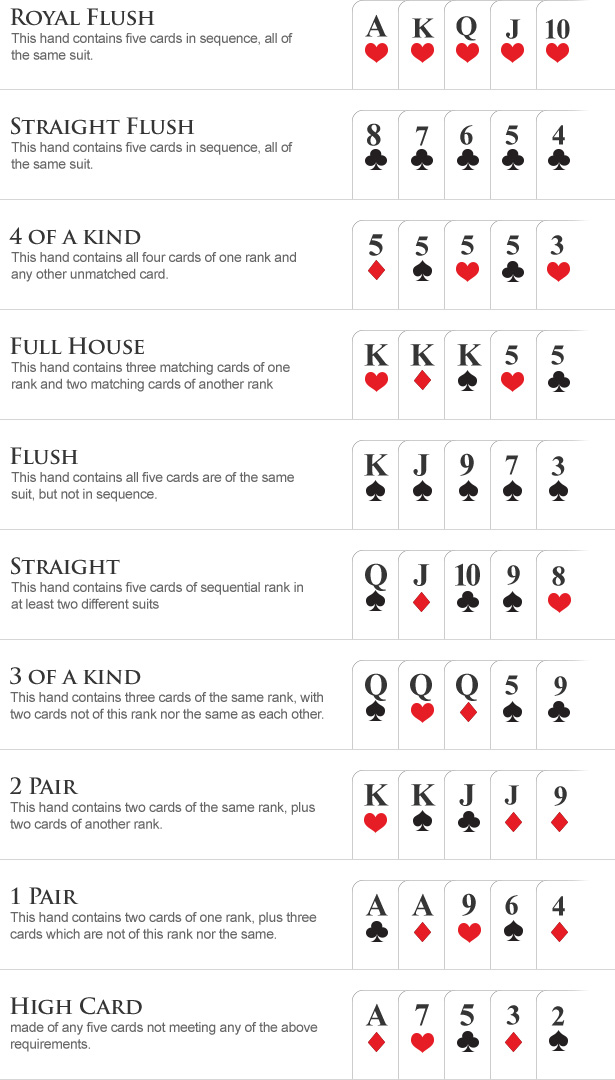
\includegraphics[width=100mm]{images/how-to-ranking.jpg}
\end{figure*}\newline 
The player with the highest ranking hand then wins the whole pot.
\subsection{Notation}
We will use the notation of [card][suit] to denote cards, for example the ace of hearts is denoted Ah, the ten of clubs is denoted Tc, and the 2 of spades is denoted 2s.
\section{Basic poker strategy}
\subsection{Expected value}
When we play poker, we are essentially making a series of decisions for chips. Of course, we may get unlucky sometimes - but anyone with a basic knowledge of probability will know that we want to maximise the \emph{expected value} of our decisions. We can apply game theory to poker, which we will do later on. However, poker is a very complex game, and it's first going to be useful to look at types of hands we could hold and what their aim is.
\subsection{Hand types - preflop}
The most common decision you (or your bot) will make in poker is to raise or fold a hand before the flop. Let's consider two hands we could be dealt preflop:\\\\
The first is a pair of aces, AsAd. \newline 
The second is the hand 7s2d. \\\\ 
The best hand of these two is clearly the pair of aces, since we already hold the highest pair possible. 7s2d is in fact very weak compared to the average poker hand; it's made of low cards, so any pair we hit is likely to be beaten by a higher one, and it also is very unlikely to make a straight or flush. So we would expect the first hand has a higher expected value, should we choose to play it. Every competent poker player will raise the first hand preflop and fold the second. There is far more to learn about preflop, but since this is a very basic guide we won't go further into it.
\subsection{Hand types - postflop}
The easiest way to learn about hand types is by considering an example. Take this board, where we have played until the turn:
\begin{figure*}[h]
    \centering
    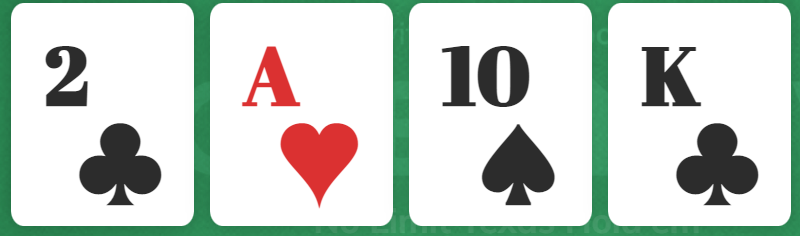
\includegraphics[width=100mm]{images/board_1.png}
\end{figure*}\newline
Let's imagine the different hands we could hold on this board. Note we can't currently hold a flush, since there are at most 2 cards of the same suit on the board. First consider the hand 10d3h. This hand on a random board would be decently strong; we have one pair of 10s, which has value at showdown. However, if we consider the \emph{relative strength} of 10d3h on this board, it is slightly weaker. This is because there are both an A and a K on the board, making it more likely our opponent will have a hand that beats ours.\\\\ Now let's consider the hand Qc8c. This hand only has 'high card' showdown value on this board. However, we have the possibility to improve to a flush if the river card is a club. This type of hand is called a 'drawing hand', where we hope to hit certain cards ("outs") to make a very strong hand. But if our draw misses, we will be left with a very bad hand. This would be a good hand to try and bluff your opponent out of the pot with by making a bet - if they fold, they likely folded a better hand than ours currently, and if they do call us, we still have a possibility of making a very strong hand. \\\\
Now imagine we've got 7s3d on this board. This hand has not made a pair, and its highest card is only 7. We have a very low chance of even making a weak one pair. Therefore this is one of the weakest hands we would have on this board, and so if we face a bet we will most likely fold.\\\\
The final hand we'll consider is the hand QcJd on this board. This hand has made a straight with the K on the turn. In fact, this is the strongest hand we can have at this current moment (the "nuts"). It's possible that this hand could not be the best possible once the river card comes; for example, if a club comes on the river we would lose to flushes. We always want to bet aggressively with the nuts to extract maximum value from our opponent. 
\subsection{Pot odds}
Pot odds are very related to the idea of maximising expected value. We're going to begin with a claim, which is that for any state of the game, there exists some probability $p$ of winning. Even if our opponent adopts a strategy that incorporates randomised behavior, this probability still exists. Given that we have some probability of winning, we can calculate an expected value. Let us say that our opponent bets an amount $c$ into a pot of size $S$. If we continue to play, the expected amount we'll win is $p \times S$, and the expected amount we'll lose is $(1-p) \times c$. Note that these amounts aren't symmetric. That's because in poker, you should consider every cost a sunk cost; that is, never worry about money committed to the pot in the past, as it is already gone. The only cost you're considering is the further cost of continuing, which you're using as some stake to win all the money in the pot. When it comes to expected value, we don't want to make a negative expected value decision - in fact, we wish to maximize expected value. Note that if the expected value is 0 , we're indifferent when it comes to folding or continuing.

The next step is to perform some algebra to separate out the probability of winning, and this gives us a cutoff for whether or not we stay in the game. We call the right hand side of the new inequality for $p$ the "pot odds:"
\[p=\frac{c}{S+c}.\]

\end{document}
